\section{Il contenuto}
Dopo aver esaminato nel dettaglio la homepage, qua di seguito verranno analizzate le pagine interne più significative e alcuni aspetti comuni in esse, come breadcrumb e ricerca. 

\subsection{Intestazione}
Ogni pagina del sito, sia homepage che interna, ha la stessa intestazione, che consta del logo, del menù e soprattutto della barra di ricerca.
\begin{figure}[!htb]
	\center{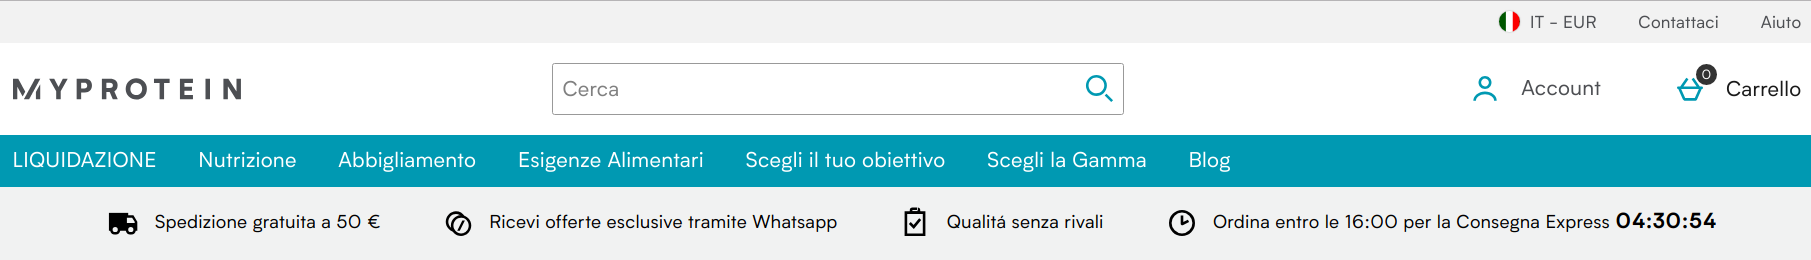
\includegraphics[width=\textwidth]
		{img/figura5.png}}
	\caption{\label{fig:figura5}} Intestazione del sito, comune a tutte le pagine.
\end{figure}


\subsection{Ricerca}
MyProtein offre centinaia di prodotti di eterogenee caratteristiche, che vanno dagl integratori ai capi di abbigliamento. E' quindi fondamentale la funzionalità di \textit{ricerca interna} che il sito offre. Essa è presente nella parte alta di tutte le pagine, ed è implementata con:
\begin{itemize}
    \item Un campo di testo, nel quale ci stanno circa 38 caratteri;
    \item Un tasto che scatena la ricerca, contenente l'icona della lente.
\end{itemize}
Le dimensioni del box di ricerca sono adeguate, considerando che la capienza minima consigliata è di circa 30 caratteri. Il tasto che scatena la ricerca, invece, ha solo l'icona della lente, senza testo. Anche se è stato dimostrato che gli utenti si trovano più a loro agio con la scritta "search" o "cerca", l'icona della lente è ormai una convenzione nel web. Finchè poi si scrive, il tasto si "evidenzia" colorandosi di bianco su sfondo blu, evidenziando il fatto che sia cliccabile, come visibile in figura 6. Inoltre, la ricerca può essere lanciata anche con il tasto "invio" della tastiera.\\
Sempre in figura 6 sono visibili i suggerimenti di ricerca, calcolati in tempo reale mentre l'utente scrive sul campo di ricerca, divisi in due tipologie:
\begin{itemize}
    \item completamento della query in base alle ricerche frequenti, nella parte superiore;
    \item prodotti più comuni suggeriti in base alla query scritta, nella parte inferiore.
\end{itemize}
Per selezionare un suggerimento si può usare il mouse (clicandoci sopra) o la tastiera (tramite le frecce direzionali e il tasto invio). Il menù a tendina in cui sono contenuti tali suggerimenti, inoltre, è fault tolerant, in quanto non si chiude se ci si sposta al di fuori di esso con il puntatore del mouse. \\
Personalmente trovo i prodotti più comuni nei suggerimenti di ricerca molto utili e, grazie ad essi, non vi è quasi mai il bisogno di utilizzare la pagina che mostra i risultati completi (che descriverò nella sezione successiva). La rappresentazione dei prodotti è scarna ma molto efficace: è presente il nome, una piccola immagine di anteprima (inutile ma graficamente piacevole), la valutazione media e, soprattutto, un'indicazione di prezzo.
\begin{figure}[!htb]
	\center{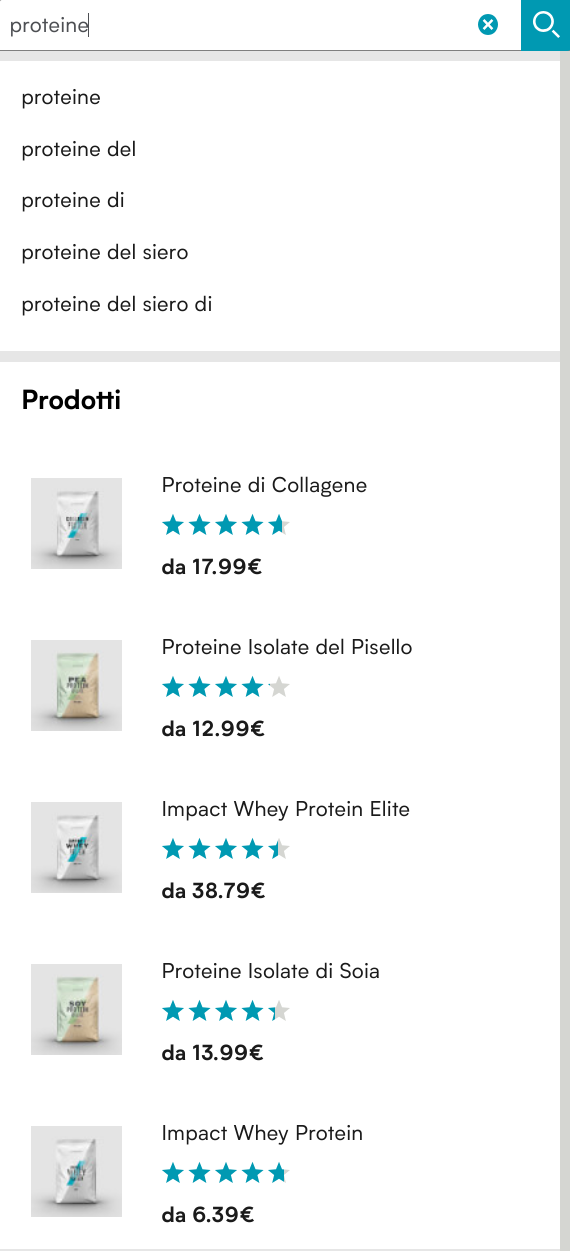
\includegraphics[width=0.5\textwidth]
		{img/figura6.png}}
	\caption{\label{fig:figura6}} Suggerimenti di ricerca.
\end{figure}

\subsection{Visualizzazione risultati}
\begin{figure}[!htb]
	\center{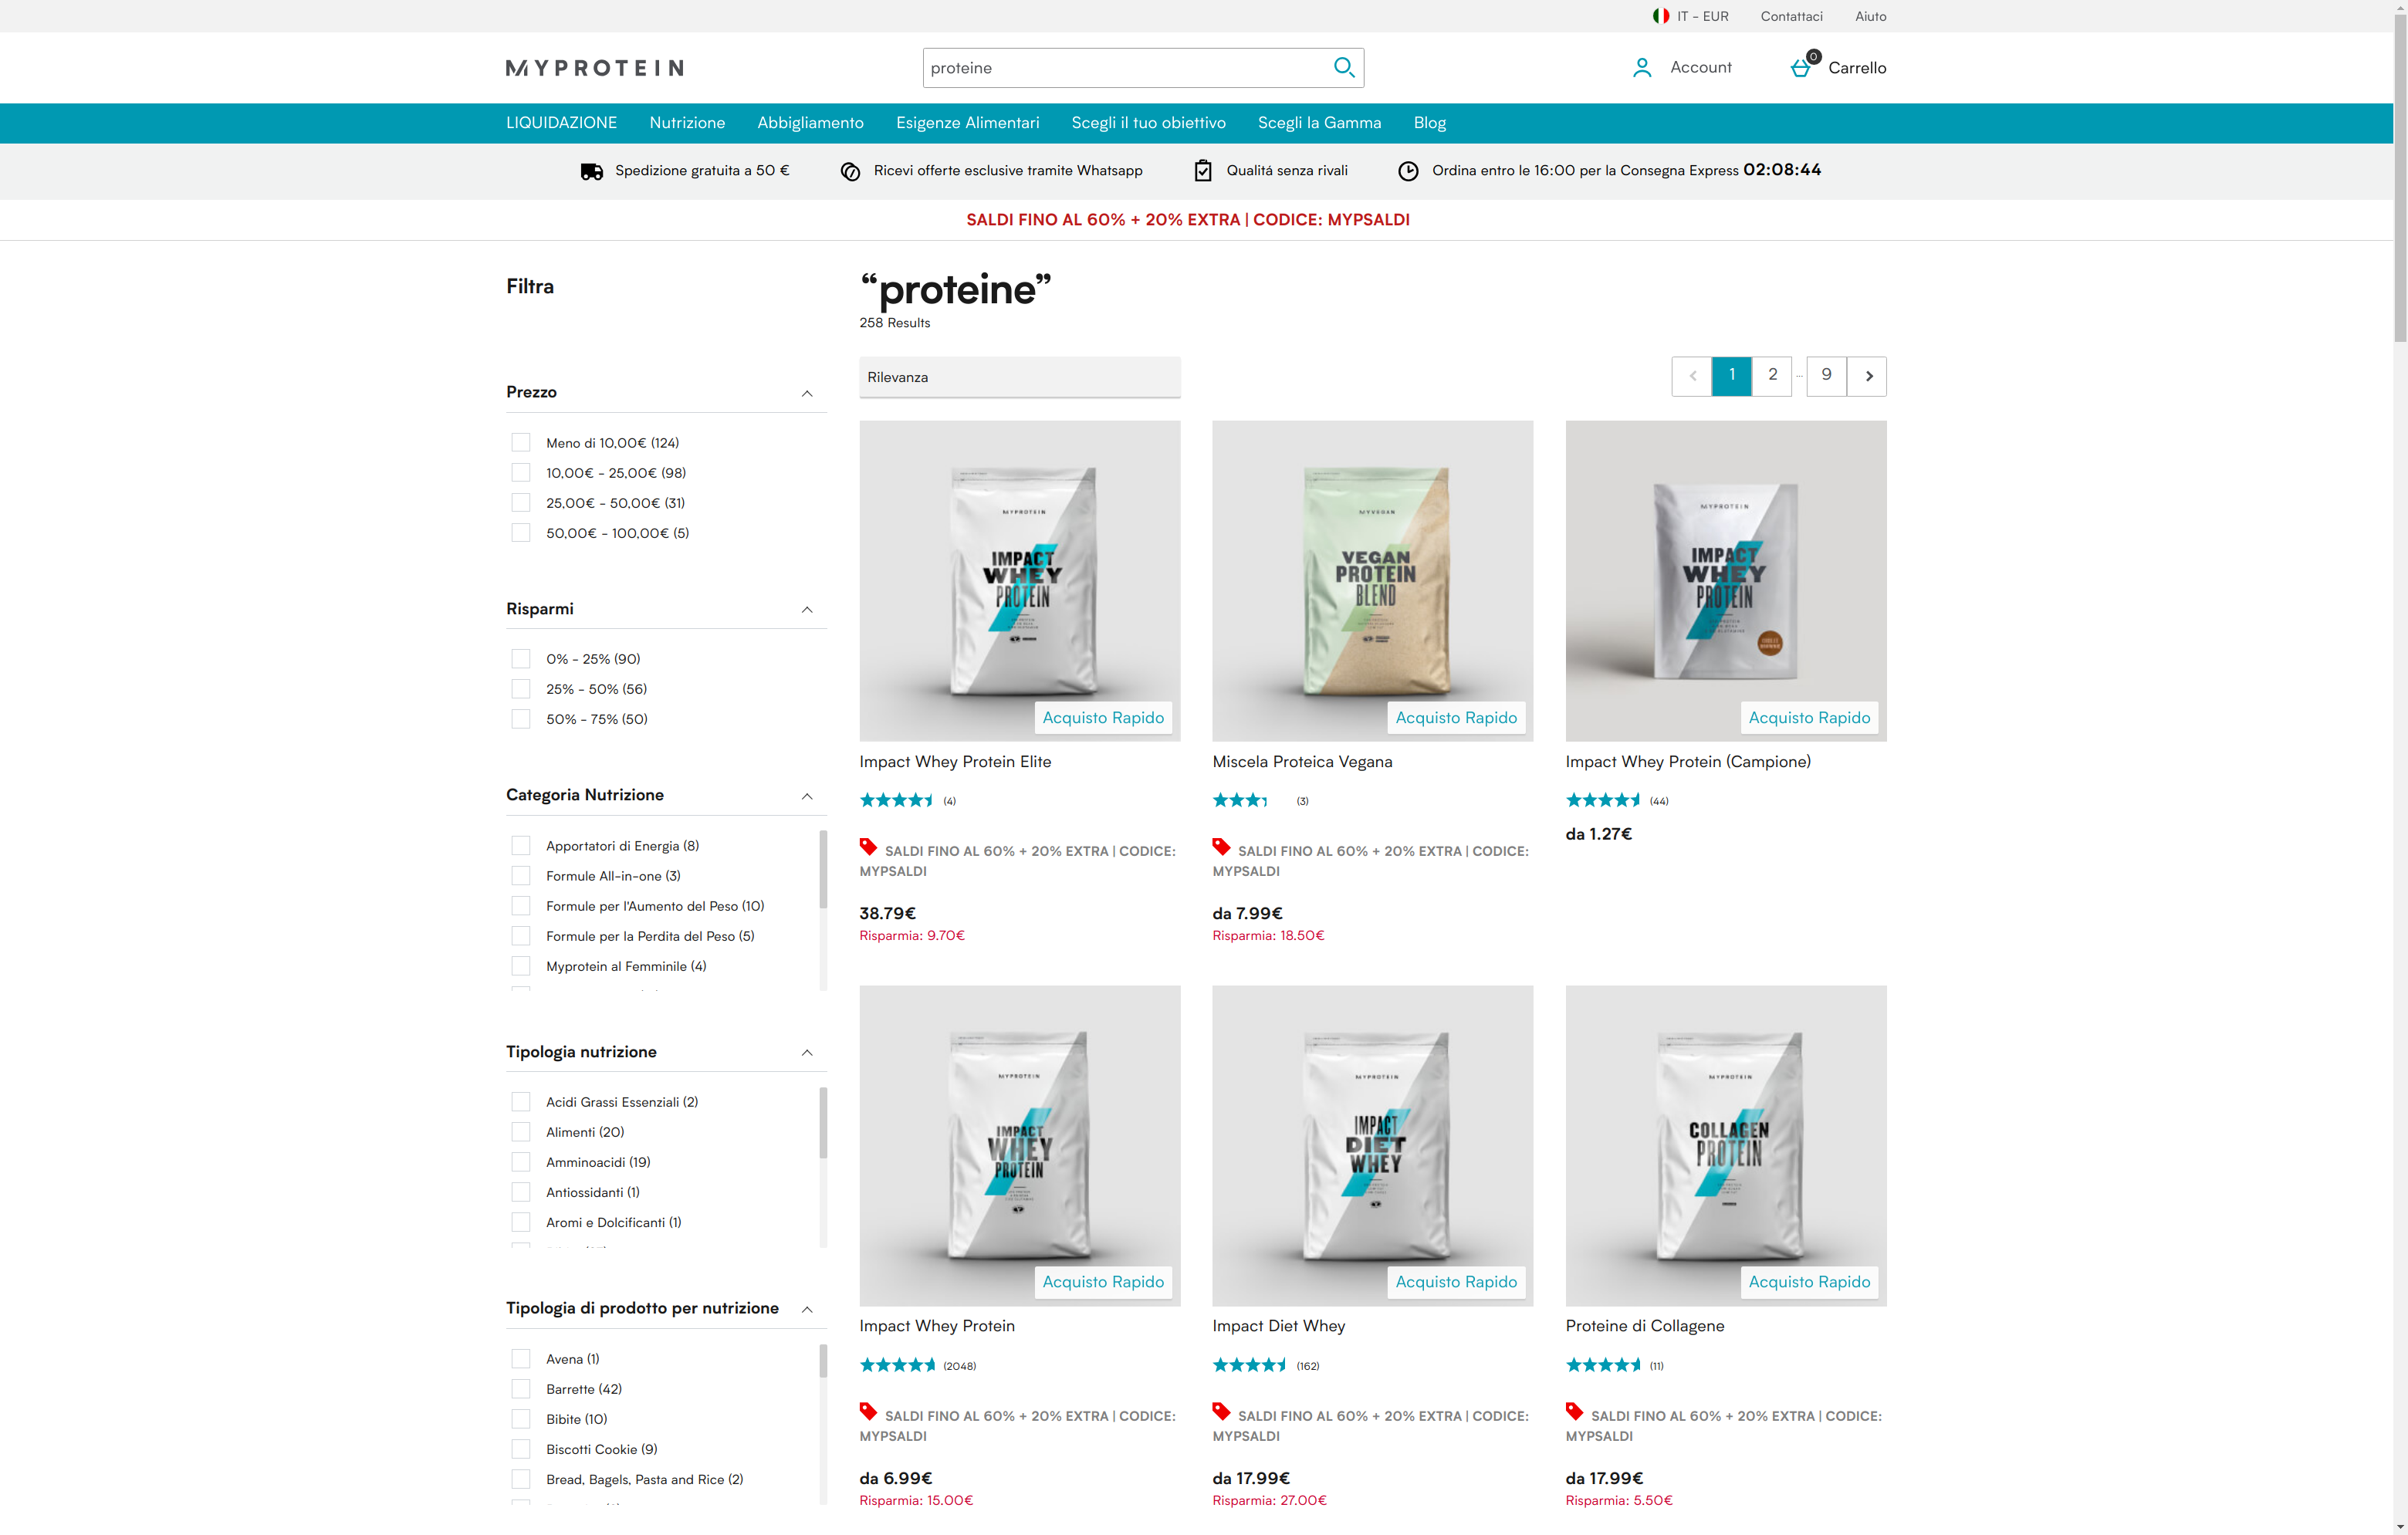
\includegraphics[width=\textwidth]
		{img/figura7.png}}
	\caption{\label{fig:figura7}} Risultati di ricerca con query "proteine".
\end{figure}
In figura 7 è rappresentata la pagina che mostra i risultati di una ricerca. Essa si compone di tre elementi fondamentali:
\begin{enumerate}
    \item prodotti risultato della ricerca;
    \item filtri avanzati;
    \item ordinamento e navigazione.
\end{enumerate}
\paragraph{Prodotti}
I risultati di ricerca sono disposti in una griglia di tre colonne, raggruppati in pagine, ciascuna contenente 30 elementi.
Per ogni prodotto è presente la foto, il nome, il rating medio (in stelle, da 0 a 5), eventuali promozioni attive/codici sconto collegati (ad esempio, in figura, "SALDI FINO AL 60\% + 20\% EXTRA | CODICE: MYPSALDI") e, soprattutto, il prezzo. Esso, seppur in caso di prodotti venduti in più varianti (ad esempio, confezione da 1kg e confezione da 2.5kg) si riferisca a quella più economica, non è un prezzo esca, ed è addirittura al lordo degli sconti che si possono applicare con gli eventuali codici sconto reperiti dal sito o dai partner: MyProtein infatti adotta la strateglia dell'\textit{affiliate marketing}, sponsorizzando degli atleti e distribuendo loro dei codici sconto da dare ai loro seguaci validi 365 giorni l'anno. Il prezzo non comprende la spedizione ma, come specificato nell'intestazione di tutte le pagine, essa è gratuita per ordini superiori ai 50 euro. \\
Ritengo che la rappresentazione dei risultati di ricerca sia stata fatta in maniera molto positiva, ad eccezione di una cosa: per entrare nel dettaglio del prodotto (e quindi aggiungerlo al carrello), si può cliccare solo sopra l'immagine dello stesso. A mio avviso sarebbe stato meglio mettere anche un tasto "Visualizza dettagli", o per lo meno rendere anche il nome del prodotto cliccabile, magari apponendoli lo stile di un link (testo sottolineato e di un colore diverso).

\paragraph{Filtri avanzati}
A lato pagina sono presenti dei filtri avanzati che consentono di specializzare la ricerca in maniera molto fine. Essi implementano il principio della ricerca vincolata dinamica ma in modo progressivo: non è necessario per forza specificare un valore per tutti i filtri, ma al cambiamento anche di uno solo di essi, i risultati vengono aggiornati.\\
A mio parere, questa funzione è realizzata in modo molto semplice, intuitivo ed efficace.

\paragraph{Ordinamento dei risultati e navigazione tra le pagine}
Nella parte alta, sopra la prima riga di prodotti, sono presenti i comandi che consentono di cambiare l'oridne in cui i risultati sono visualizzati, ma anche di muoversi tra le pagine di ricerca. Poter ordinare i prodotti per prezzo (crescente o decrescente), per rilevanza, per popolarità ecc.. è cosa gradita. Inoltre, il fatto che i pulsanti di navigazione tra una pagina dei risultati e l'altra siano ripetuti anche nella parte alta dello schermo li rende sempre prontamente raggiungibili.

\begin{figure}[!htb]
	\center{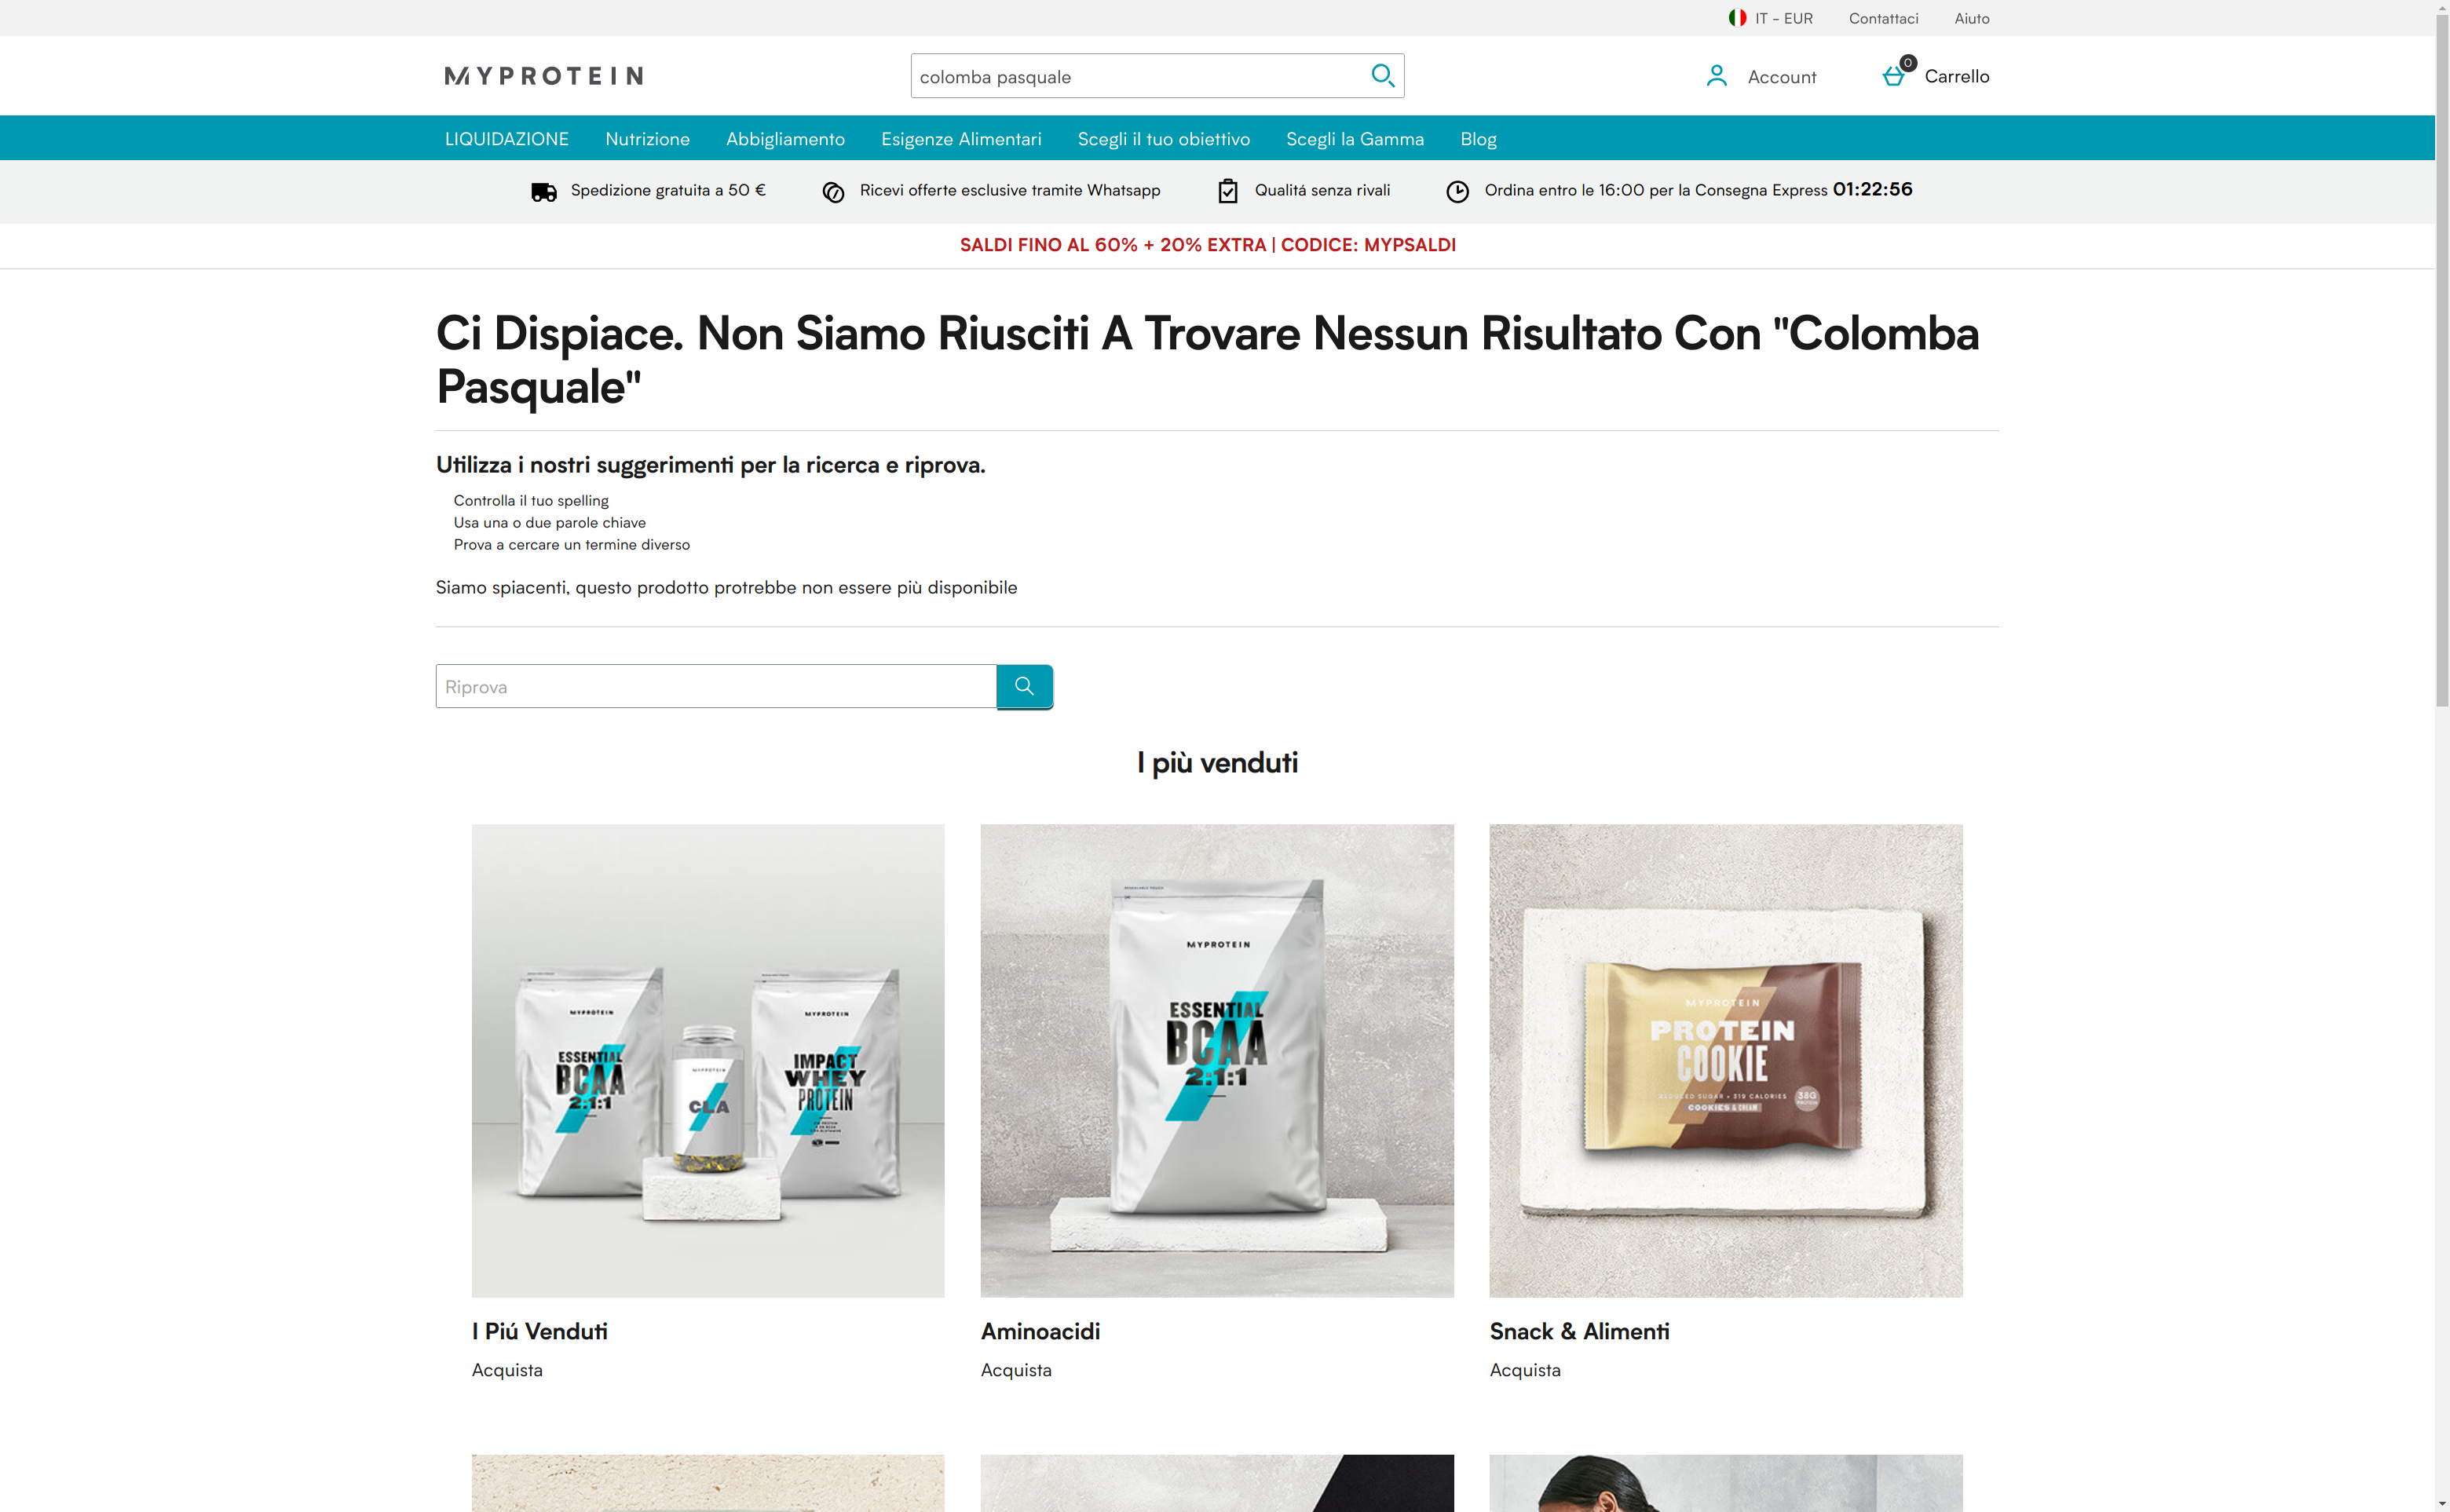
\includegraphics[width=\textwidth]
		{img/figura8.png}}
	\caption{\label{fig:figura8}} Pagina di ricerca senza esito.
\end{figure}

In caso non ci siano prodotti che soddisfino i criteri di ricerca dell'utente, il fatto li viene comunicato tramite una pagina che fornisce anche una carrellata di prodotti più venduti, ai quali è statisticamente più facile che l'internauta sia interessato.

\subsection{Dettaglio prodotto}
\begin{figure}[!htb]
	\center{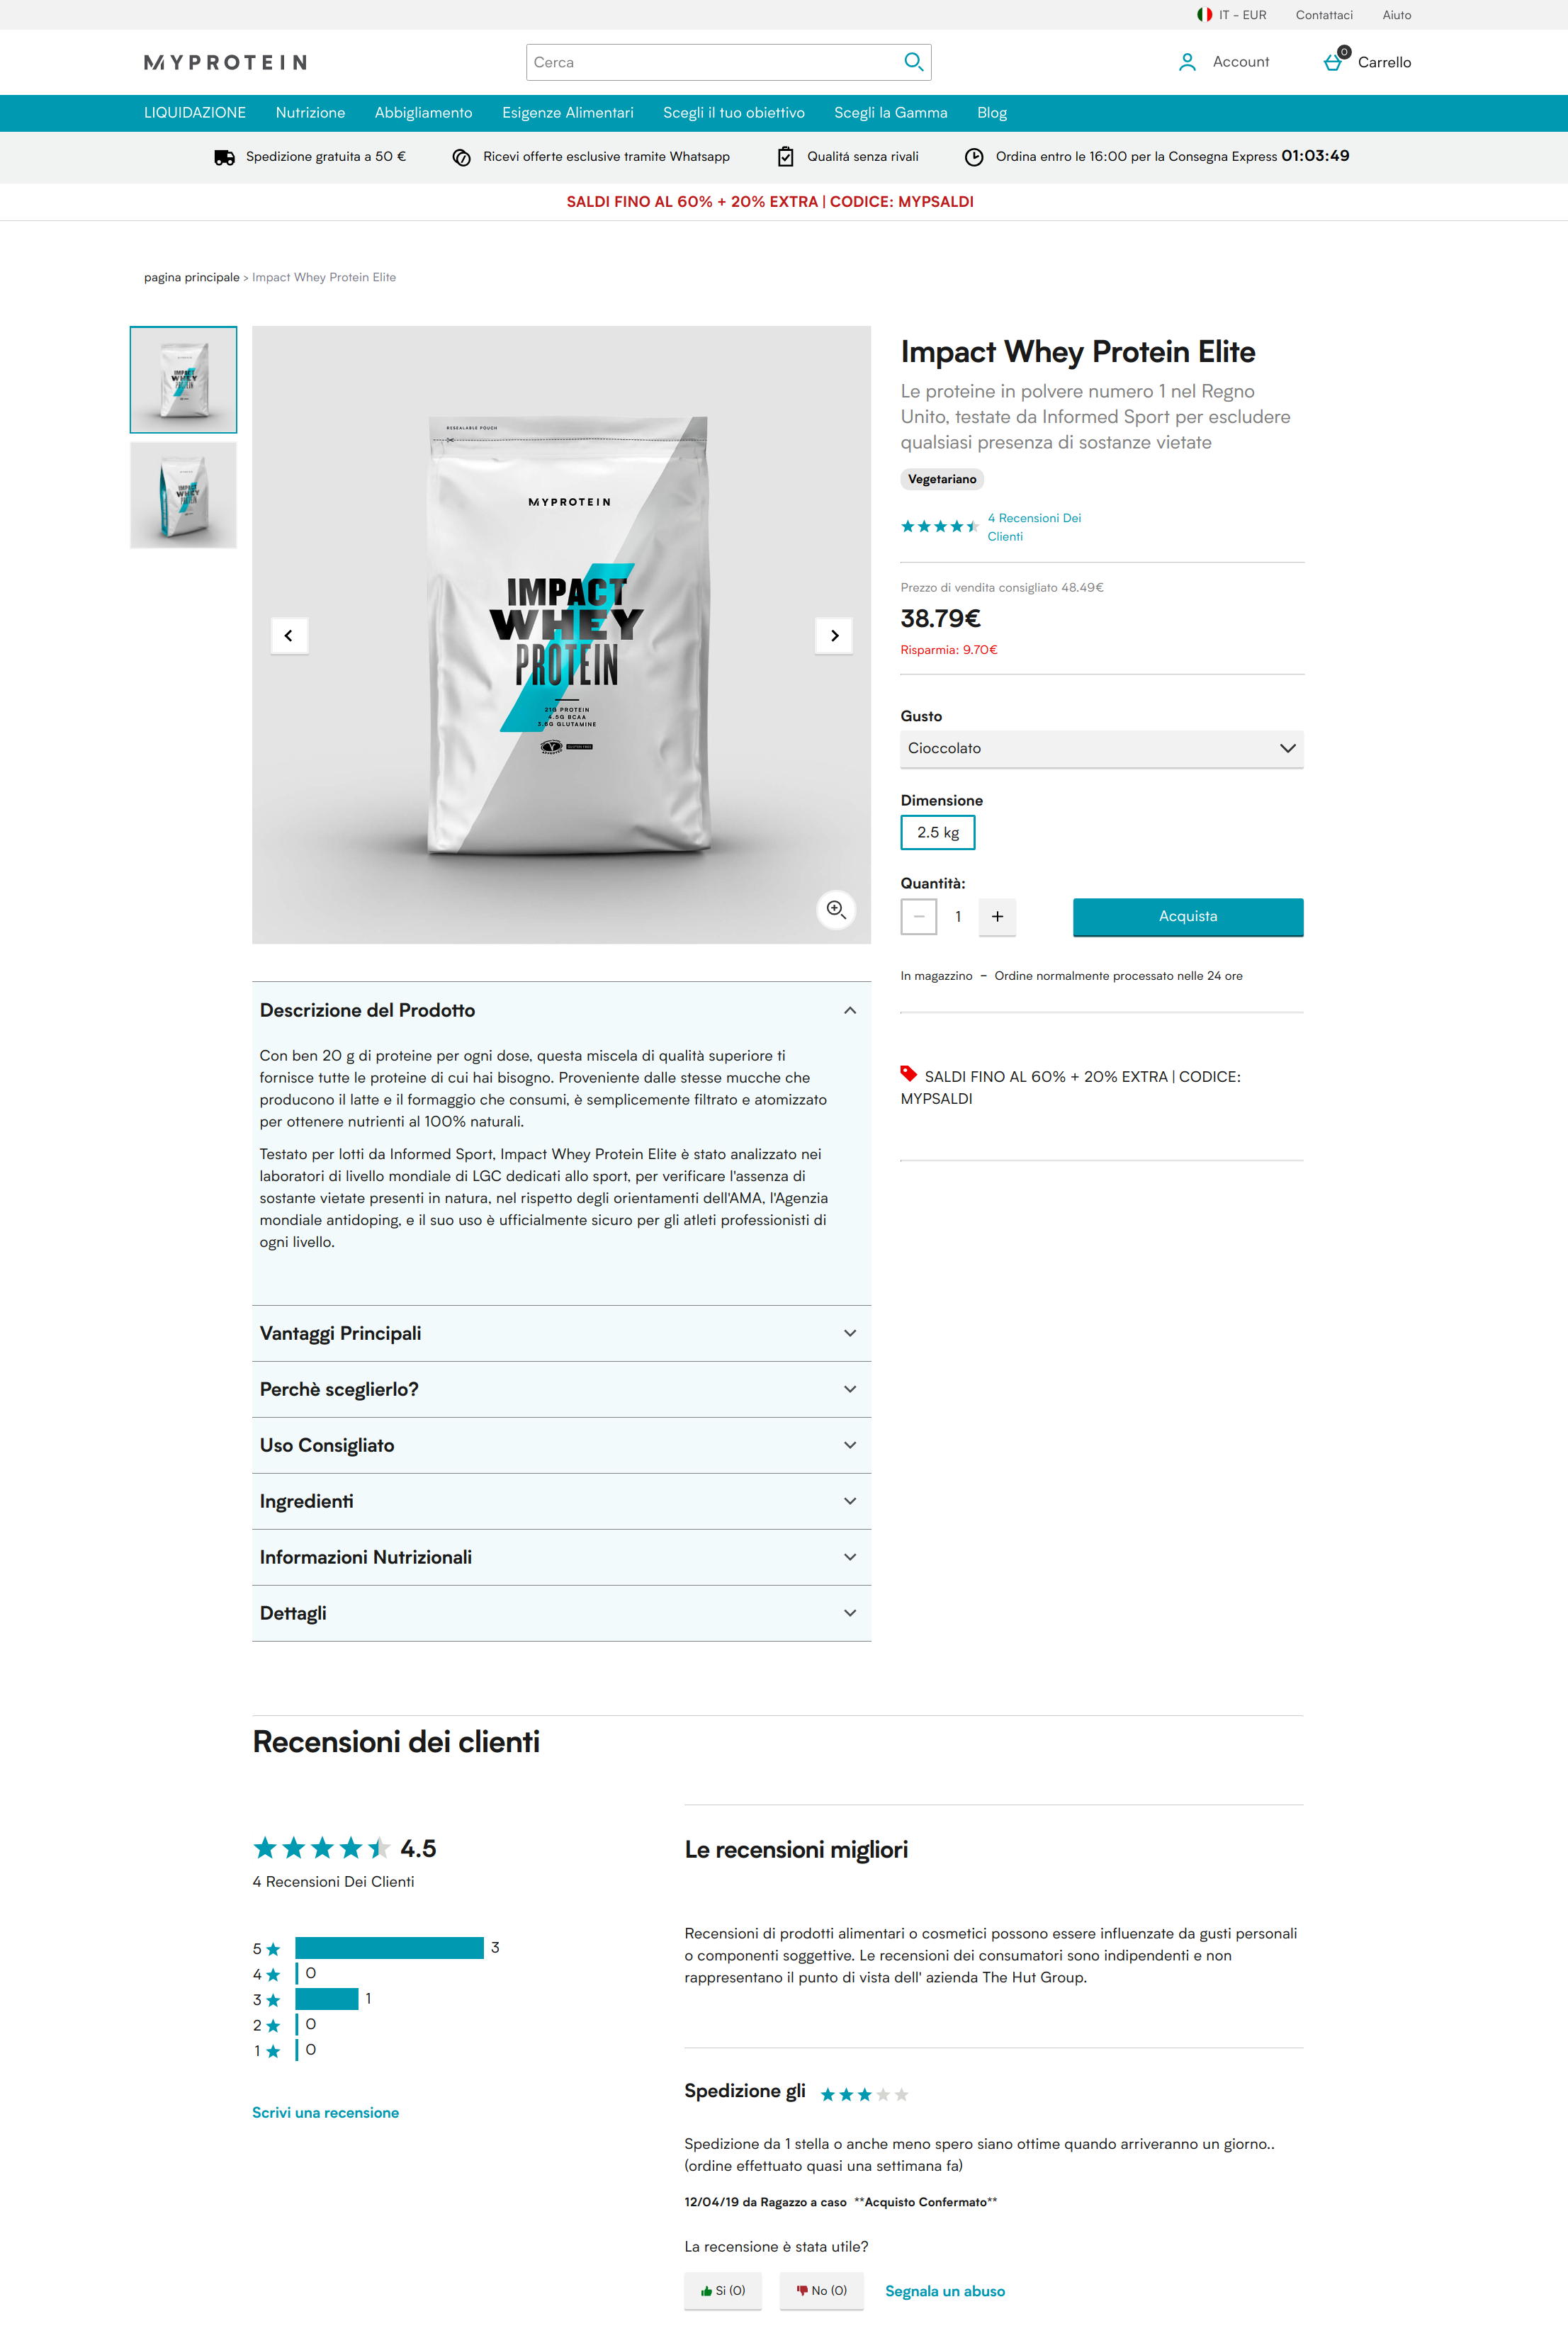
\includegraphics[width=.71\textwidth]
		{img/figura9.png}}
	\caption{\label{fig:figura9}} Dettaglio di un prodotto. N.b.: l'area catturata nell'immagine è più della porzione visibile.
\end{figure}
Questa pagina presenta un prodotto nel dettaglio. Contiene il suo nome, il prezzo, le varianti acquistabili (in gusto e dimensione, ad esempio), la descrizione dettagliata, le foto, i commenti/recensioni e un set di prodotti correlati suggeriti (non presenti nello screenshot).\\ 
L'articolo è rappresentato graficamente in 2D tramite delle foto che lo ritraggono con diverse angolature; tali foto possono essere anche zoomate/visualizzate a tutto schermo. Trovo positivo che non sia stata adottata una soluzione 3D, che avrebbe inutilmente causato del sovraccarico cognitivo anche perché onestamente ritengo inutile poter vedere più di un paio di angolazini di un sacchetto di integratori (l'importante non è la grafica del sacchetto, ma il contenuto!!).\\
Il prezzo del prodotto è rappresentato per singola unità, al lordo degli sconti e al netto della spedizione. Cambiando variante (ad esempio selezionando un gusto diverso o, quando disponibile, una dimensione diversa) esso si aggiorna automaticamente. Qualche riga sotto di esso è presente anche la disponibilità, che da un'idea del tempo necessario all'evasione dell'ordine.\\
La parte centrale della pagina è occupata dalla descrizione delle caratteristiche dell'articolo, quali ingredienti, usi consigliati, informazioni nutrizionali (molto importanti in prodotti del genere). Sebbene esse siano contenute in un menù a fisarmonica, quindi obblighino di fatto l'utente ad un click in più per accedere all'informazione desiderata, questa scelta permette di mantenere la pagina molto ordinata e, di conseguenza, diminuire lo sforzo computazionale necessario all'utente per trovare l'informazione desiderata.\\
Nella parte inferiore della pagina sono presenti le recensioni effettuate da altri clienti, che possono aiutare nel valutare l'efficacia di un prodotto (anche se, soprattutto per gli alimenti/integratori, andrebbero prese con le pinze) e i prodotti correlati, utili se non si ha un'idea ben precisa delle proprie necessità.\\
Infine, ultimo ma non ultimo, nella parte alta della pagina si trova il pulsante "Acquista". Alla pressione, esso rivela una finestra di dialogo (si veda figura 10) che riepiloga il prodotto che si è appena inserito nel carrello (prezzo x quantità) e il totale parziale dello stesso. Dentro la finestra sono presenti anche altri due pulsanti, "Cassa" (che permette di concludere l'ordine e pagare) e "Continua ad acquistare", che chiude la finestra modale. La criticità maggiore che ho individuato è l'assenza di via di fuga, a meno della pressione del tasto "Continua ad acquistare" o della "X" posta in alto a destra per chiudere la finestra di dialogo. Infatti, il click al di fuori dell'area della modal non la chiude, e la pressione del tasto "Indietro" del browser fa uscire dalla pagina del prodotto. Personalmente, per quanto comoda, eviterei l'uso di una finestra modale, o quantomeno implementerei una via di fuga, come la chiusura se viene premuta un'area al di fuori della finestra.
\begin{figure}[!htb]
	\center{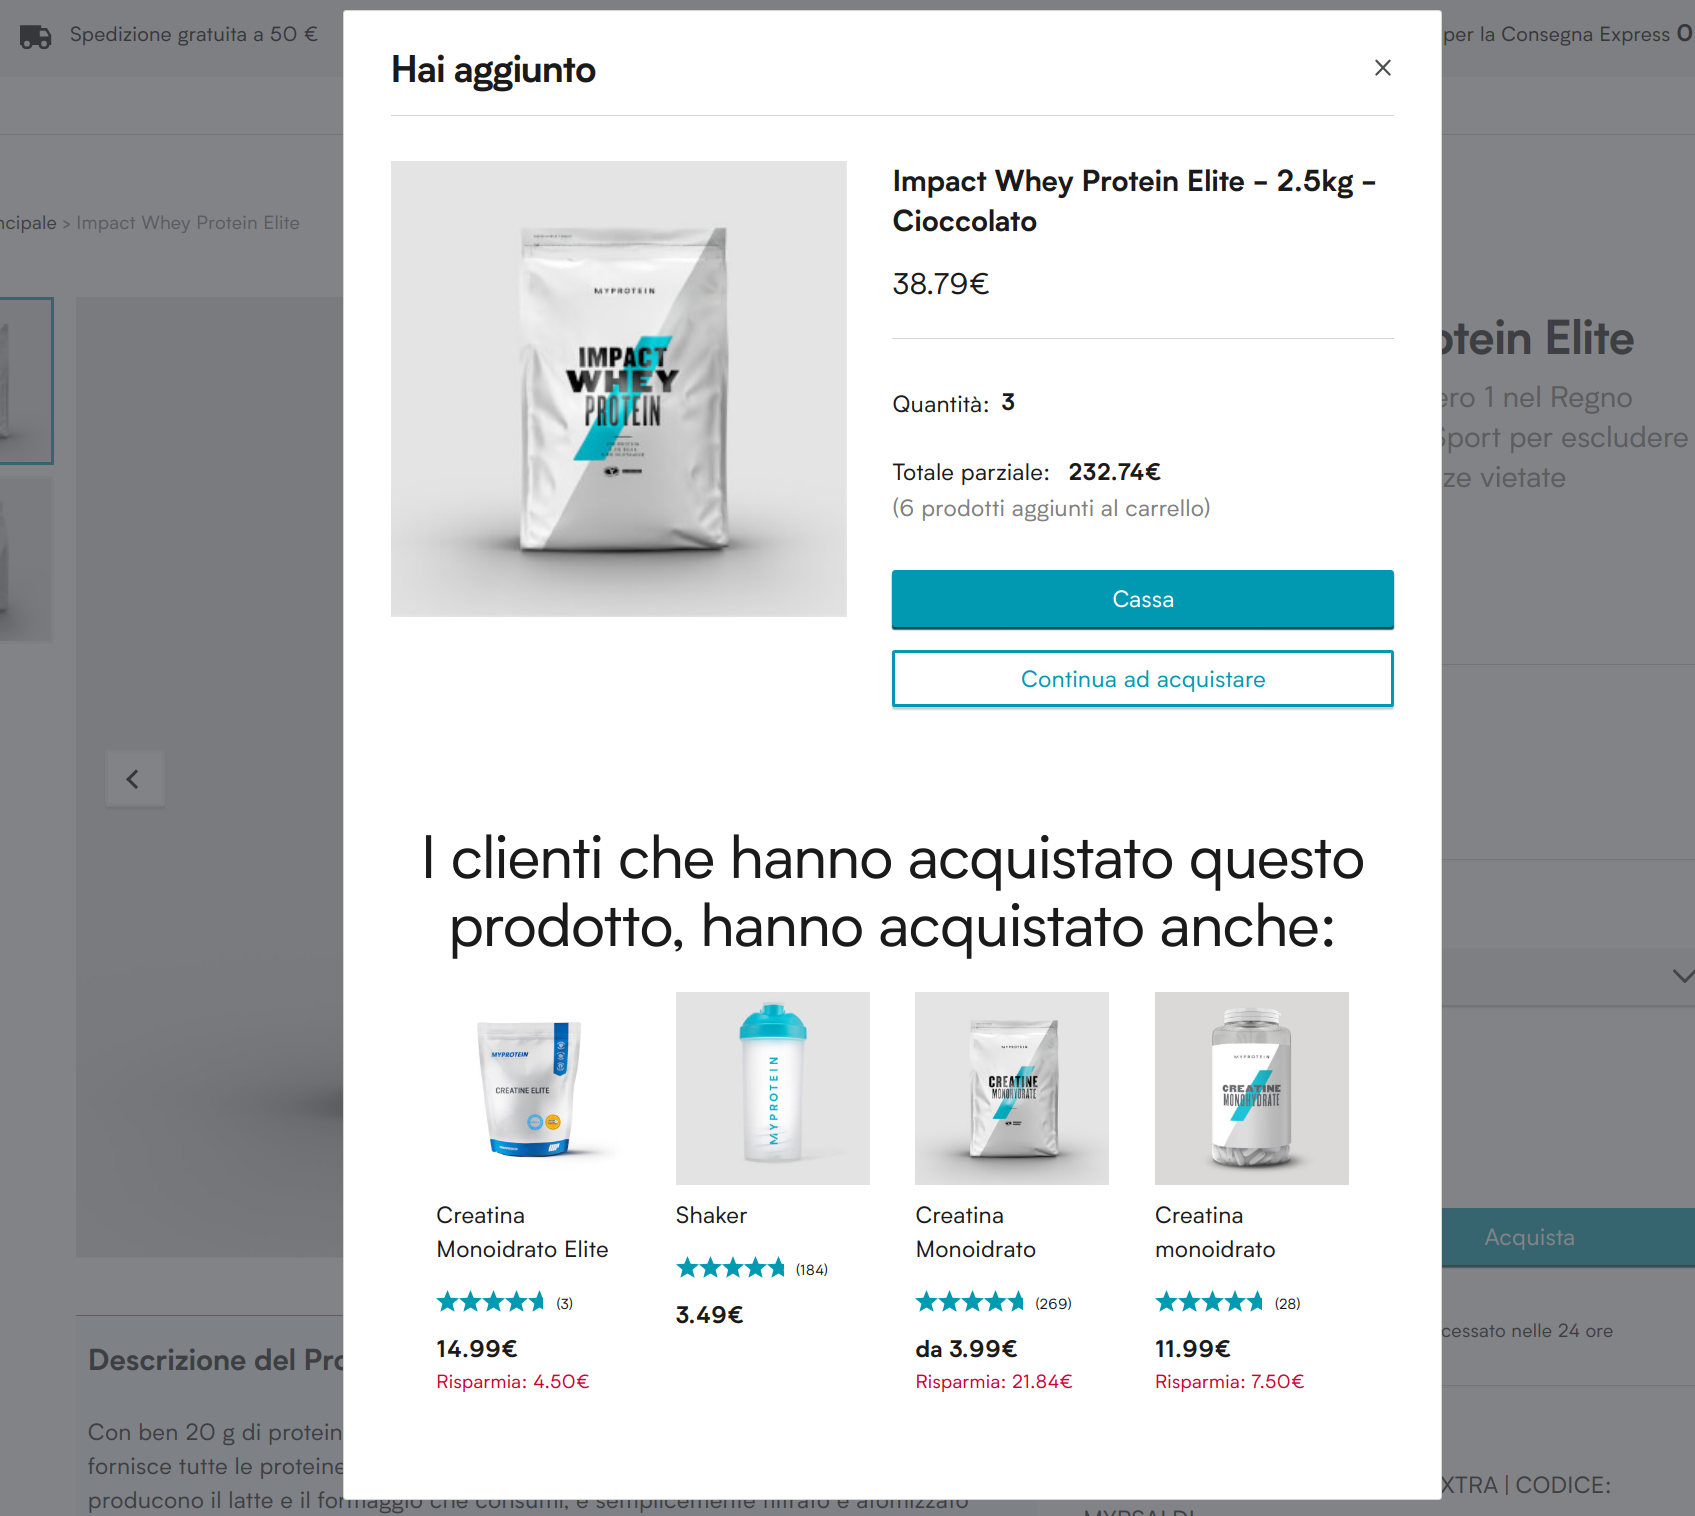
\includegraphics[width=\textwidth]
		{img/figura10.png}} 
	\caption{\label{fig:figura10}} Finestra modale che compare dopo la pressione del tasto "Acquista".
\end{figure}\\

\pagebreak
\subsection{Cassa}
\begin{figure}[!htb]
	\center{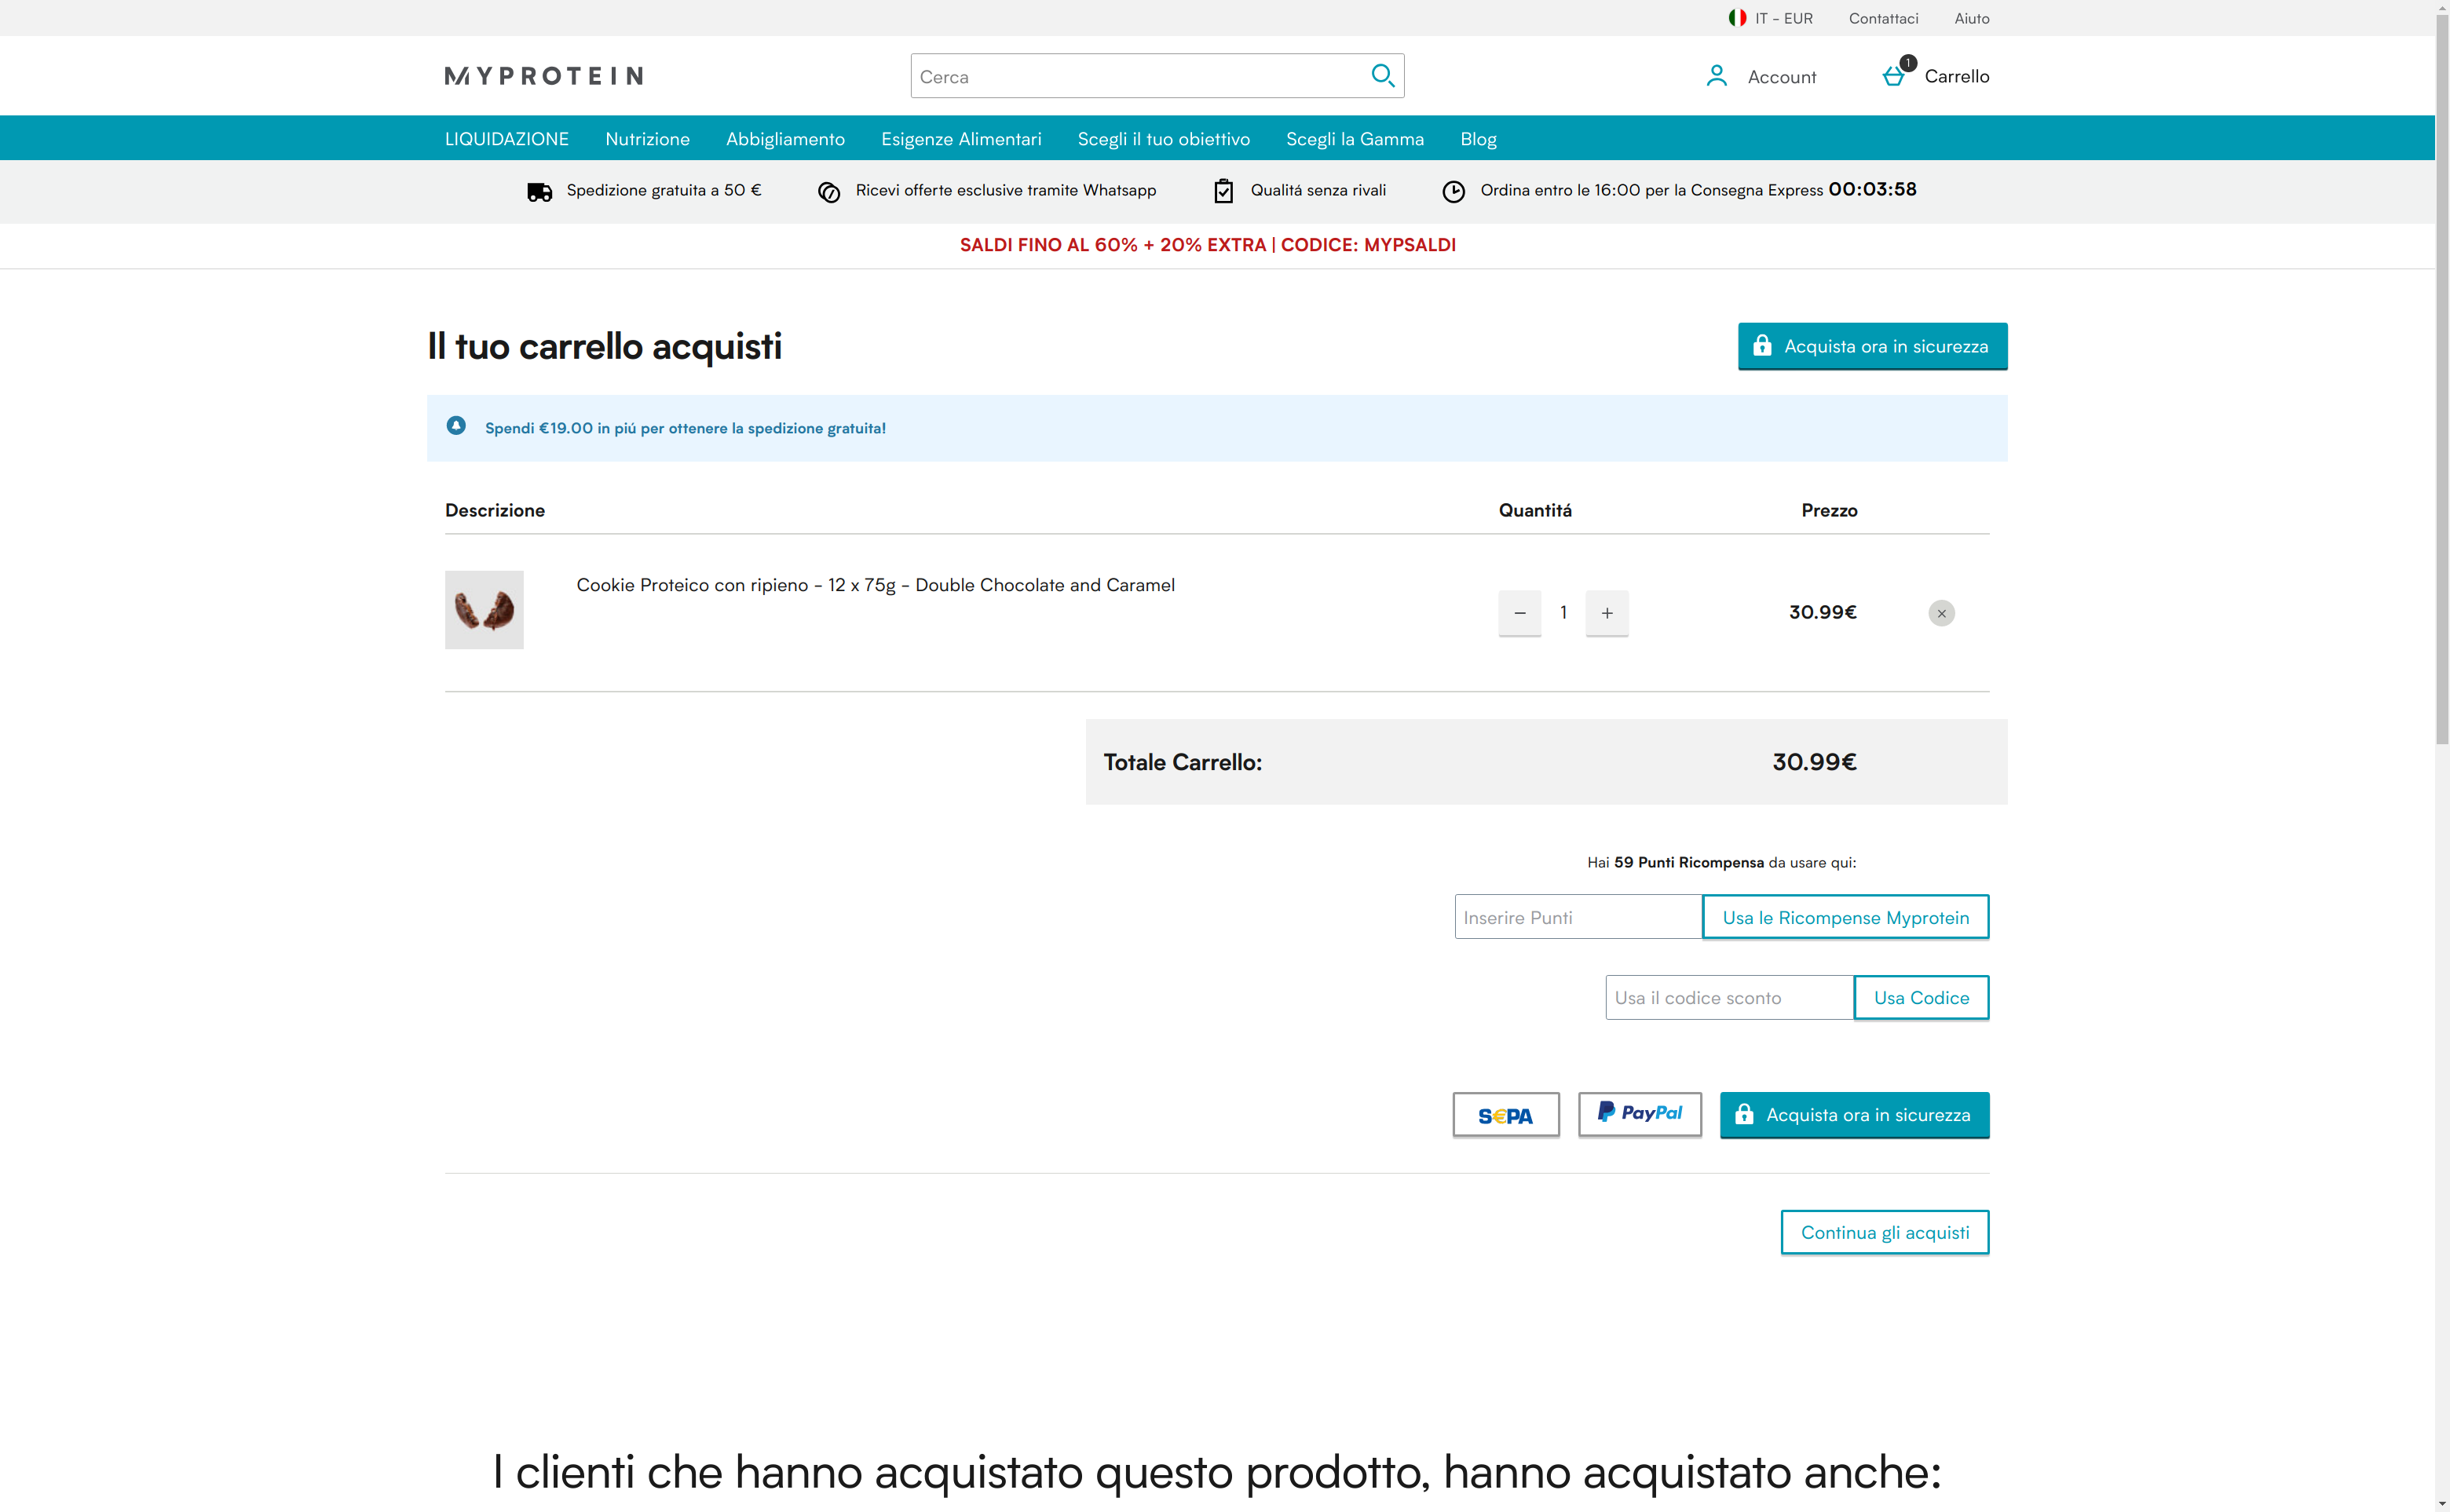
\includegraphics[width=\textwidth]
		{img/figura11.png}} 
	\caption{\label{fig:figura11}} Cassa.
\end{figure}
Questa pagina, accessibile anche senza aver effettuato alcun tipo di registrazione/login, offre il riepilogo degli articoli inseriti nel carrello e contiene i collegamenti necessari a confermare l'ordine e quindi pagare. La critica che muovo a questa pagina è l'assenza dei costi di spedizione calcolati nel totale. Ho scelto apposta un prodotto di importo inferiore ai 50 \euro (30.99), e comunque nel totale non compaiono le spese di spedizione. Questa "negligenza" è mitigata dal fatto che, nella parte alta della pagina, compare un messaggio con scritto "Spendi 19.00\euro \! in più per la spedizione gratuita!", anche se suggerirei di menzionare in ogni caso l'importo della spedizione (anche solo stimato) allo stato attuale del carrello.

\pagebreak
\subsection{Errore 404}
\begin{figure}[!htb]
	\center{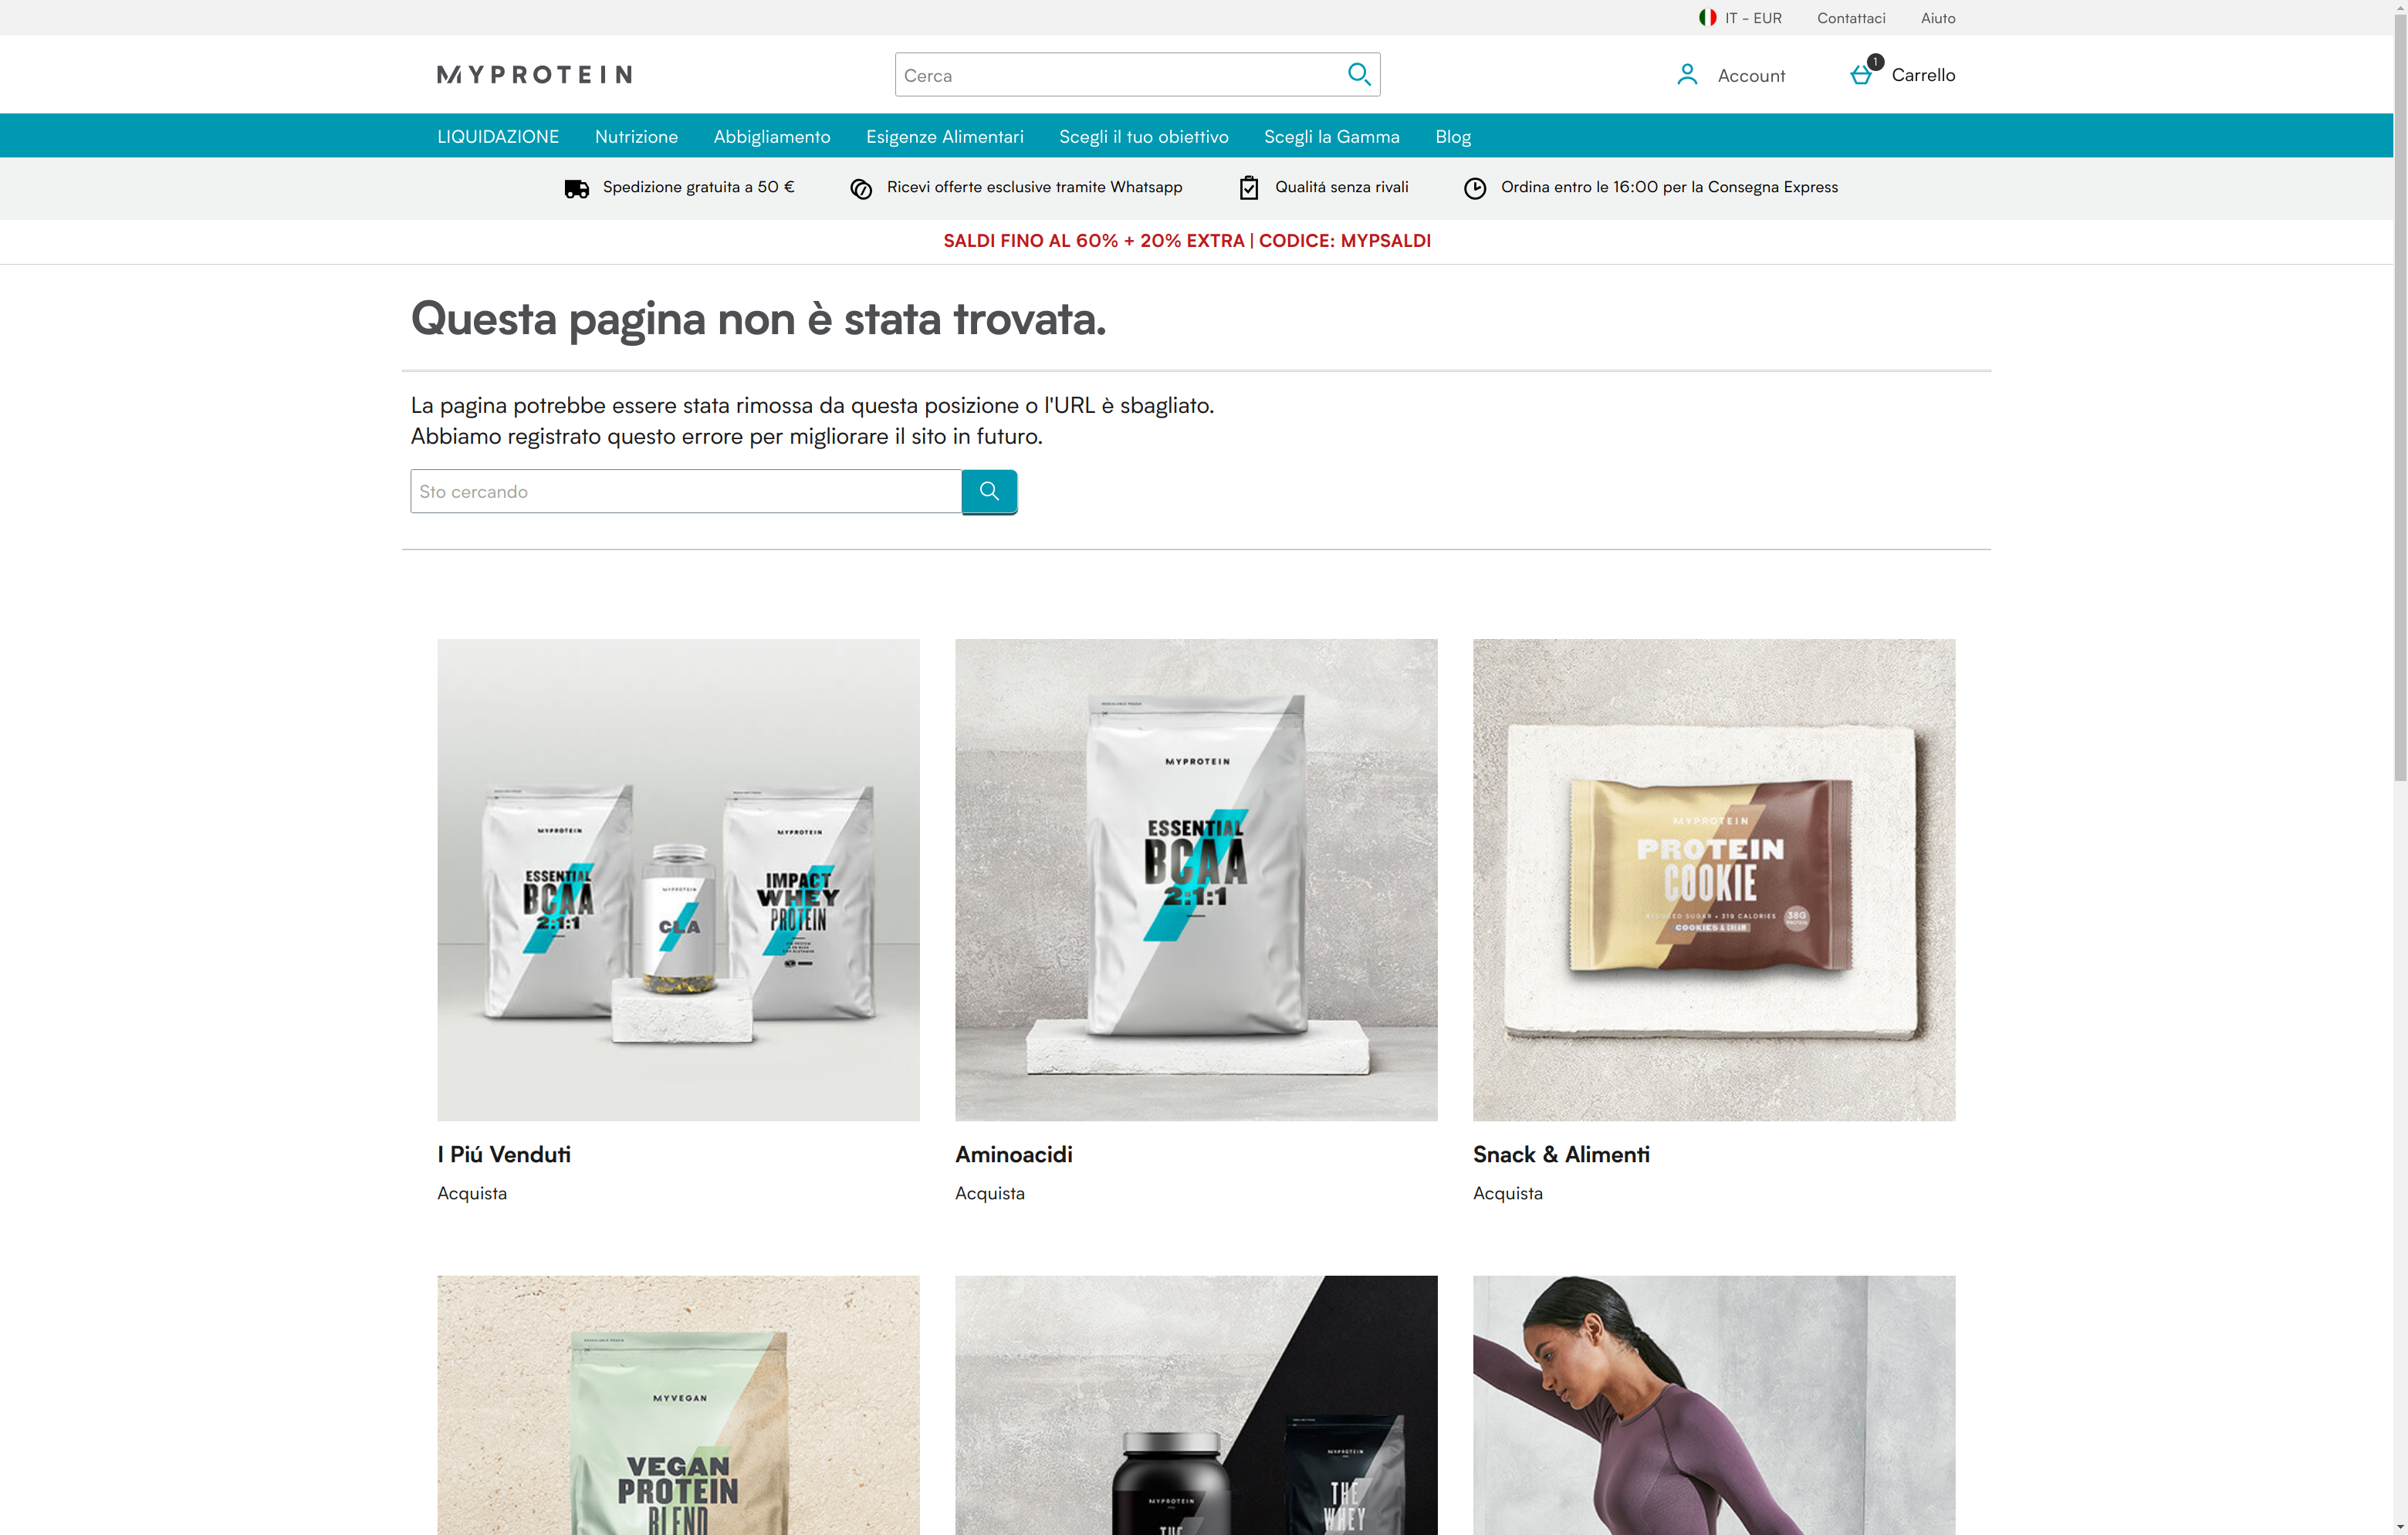
\includegraphics[width=\textwidth]
		{img/figura12.png}} 
	\caption{\label{fig:figura12}} Pagina di errore 404.
\end{figure}
La pagina in figura 12 rappresenta quella che si ottiene in caso di errore 404. L'implementazione adottata secondo me è molto buona: l'utente viene informato sull'errore, rassicurato ("Abbiamo registrato questo errore per migliorare il sito in futuro") e si trova davanti una barra di ricerca (utile anche se ridondante) e l'elenco dei prodotti di maggior successo. L'esperienza dell'utente è nel complesso buona e personalmente non ho miglioramenti da suggerire.

\subsection{Menù e breadcrumb}
Il menù del sito, in termini di usabilità, lo definirei "amore ed odio", e adesso cercherò di spiegare il perché. 
Iniziando subito con gli aspetti negativi, nel sito in realtà ci sono due menù: uno all'inizio (visibile in figura \ref{fig:figura4}, che chiamerò "Menu A") uno alla fine di ogni pagina (riportato in figura \ref{fig:figura13}, che chiamerò "Menu B"). Sebbene molti siti adottino uno sdoppiamento simile, rendendolo quasi uno standard \textit{de-facto}, ritengo disorientante avere due menù simili che, di primo acchitto possono sembrare simili, ma in realtà presentano numerose differenze sia in termini contenutistici che di interazione. Per portare un esempio, la sezione "chi siamo" è contenuta solo nel "bottom menù", mentre quella "Prodotti" sia nell'header che nel footer. Tuttavia, se nel menù in figura \ref{fig:figura4} ogni categoria di prodotto ha un sottomenù ordinato e organizzato per sezioni, in quello della figura \ref{fig:figura13} tale funzionalità si perde. Ciò comporta che, se voglio ad esempio selezionare il prodotto "BCAA Integratori":
\begin{itemize}
	\item Nel "Menù A" è sufficiente posizionare il mouse sopra la voce "Nutrizione", recarsi nella colonna "Amminoacidi" e cliccare su "BCAA Integratori" (totale click realizzati: 1);
	\item Nel "Menù B", se si clicca sulla voce "Nutrizione", si viene reindirizzati alla pagina "Proteine", che non contiene in alcun modo la categoria di prodotto "BCAA Integratori". Bisognerà pertanto o usare la funzionalità del cerca o usare il "Menù A" come descritto nel punto precedente. Onestamente, questa cosa la trovo assurda.
\end{itemize}
Proporrei pertanto o di eliminare completamente il "Menu B" o quantomeno di rendere le voci ridondanti effettivamente ridondanti, ovvero rendendole capaci di raggiungere le stesse pagine.
\begin{figure}[!htb]
	\center{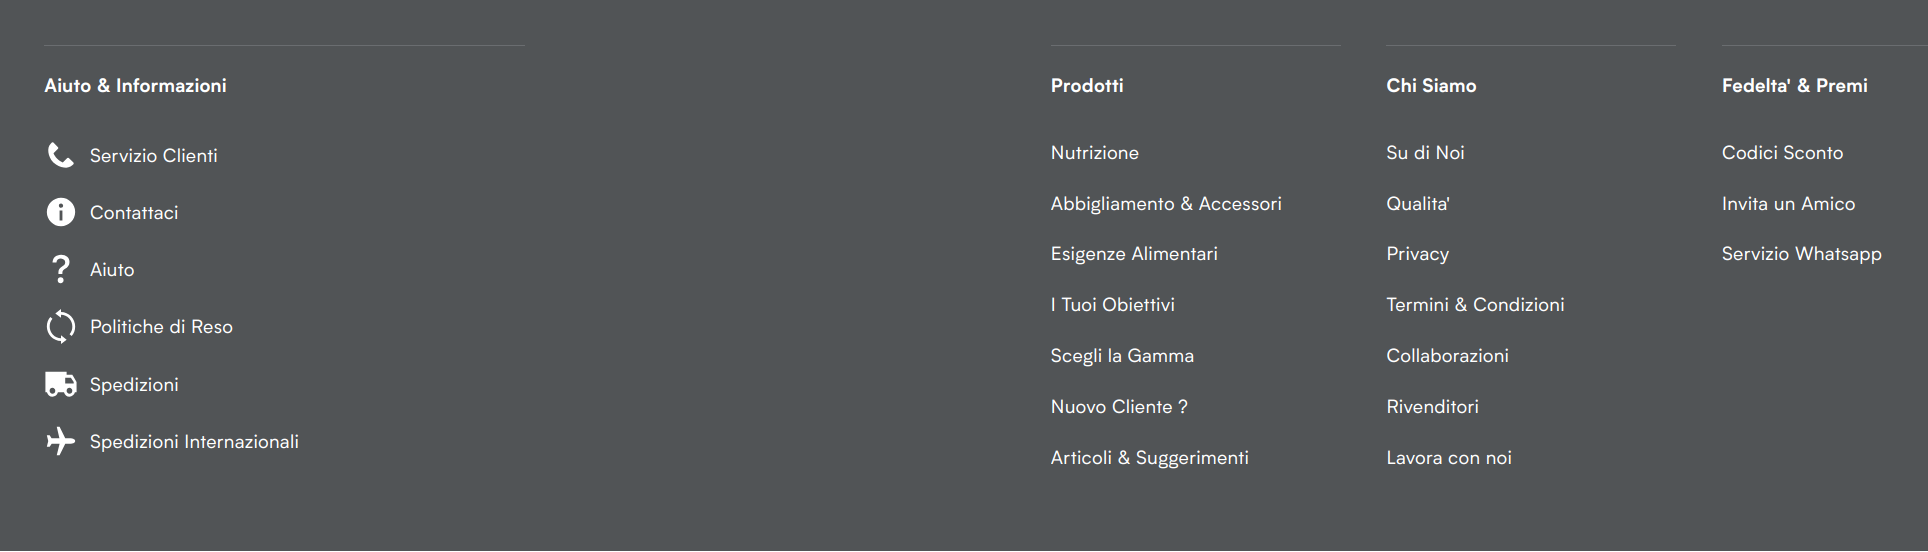
\includegraphics[width=\textwidth]
		{img/figura13.png}} 
	\caption{\label{fig:figura13}} Menù nel footer di ogni pagina.
\end{figure}\\
Aspetti positivi del menù (quantomeno del "Menù A") sono invece l'organizzazione delle voci/sottovoci e fault tolerance, di cui ho già parlato in sezione \ref{paragraph:how}.\\
Un altro elemento presente nel sito è la breadcrumb di tipo "\textit{location}", che definirei un'occasione mancata. Il problema sta nel fatto che è implementata solo in due tipologie di pagine del sito (risultati di ricerca e dettaglio prodotto), e presenta un'incongruenza nel comportamento. Poniamo che dal menù "Nutrizione" clicchi sulla voce "Proteine -> Latte e Caseina": vengo portato ad una pagina, simile in tutto e per tutto a quella dei risultati di ricerca riportata in figura \ref{fig:figura7}. La breadcrumb riporta correttamente il percorso "pagina principale > Nutrizione > Proteine > Proteine del latte e caseina". Se però clicco sul primo risultato di ricerca ("Caseina a rilascio prolungato"), la breadcrumb riporterà "pagina principale > Caseina a rilascio prolungato", perdendo informazioni preziose sul contesto. Per evitare questo, secondo me sarebbe stato meglio implementare una breadcrumb di tipo "\textit{path}".